\documentclass[10pt,ignorenonframetext,]{beamer}
% \setbeamertemplate{caption}[numbered]
% \setbeamertemplate{caption label separator}{: }
% \setbeamercolor{caption name}{fg=normal text.fg}
\usepackage{lmodern}
\usepackage{amssymb,amsmath}
\usepackage{ifxetex,ifluatex}
\usepackage{fixltx2e} % provides \textsubscript
\ifnum 0\ifxetex 1\fi\ifluatex 1\fi=0 % if pdftex
  \usepackage[T1]{fontenc}
  \usepackage[utf8]{inputenc}

% add math tools
\usepackage{mathtools}

 % add under bar
\usepackage{accents}
\newcommand{\ubar}[1]{\underaccent{\bar}{#1}}

% argmax/argmin
\DeclareMathOperator*{\argmax}{arg\,max}
\DeclareMathOperator*{\argmin}{arg\,min}

% vectors
\usepackage{bm}
\usepackage{bbm}

% backup slides
\usepackage{appendixnumberbeamer}

% drop captions
% \renewcommand \caption [2][]{}

\usepackage{changepage}

\else % if luatex or xelatex
  \ifxetex
    \usepackage{mathspec}
  \else
    \usepackage{fontspec}
  \fi
  \defaultfontfeatures{Ligatures=TeX,Scale=MatchLowercase}
  \newcommand{\euro}{€}
\fi
% use upquote if available, for straight quotes in verbatim environments
\IfFileExists{upquote.sty}{\usepackage{upquote}}{}
% use microtype if available
\IfFileExists{microtype.sty}{%
\usepackage{microtype}
\UseMicrotypeSet[protrusion]{basicmath} % disable protrusion for tt fonts
}{}
\usepackage{graphicx,grffile}
\makeatletter
\def\maxwidth{\ifdim\Gin@nat@width>\linewidth\linewidth\else\Gin@nat@width\fi}
\def\maxheight{\ifdim\Gin@nat@height>\textheight0.8\textheight\else\Gin@nat@height\fi}
\makeatother
% Scale images if necessary, so that they will not overflow the page
% margins by default, and it is still possible to overwrite the defaults
% using explicit options in \includegraphics[width, height, ...]{}
\setkeys{Gin}{width=\maxwidth,height=\maxheight,keepaspectratio}

% Comment these out if you don't want a slide with just the
% part/section/subsection/subsubsection title:
\AtBeginPart{
  \let\insertpartnumber\relax
  \let\partname\relax
  \frame{\partpage}
}
\AtBeginSection{
  \let\insertsectionnumber\relax
  \let\sectionname\relax
  \frame{\sectionpage}
}
\AtBeginSubsection{
  \let\insertsubsectionnumber\relax
  \let\subsectionname\relax
  \frame{\subsectionpage}
}

\setlength{\emergencystretch}{3em}  % prevent overfull lines
\providecommand{\tightlist}{%
  \setlength{\itemsep}{0pt}\setlength{\parskip}{0pt}}
\setcounter{secnumdepth}{0}

\title{Illegal Drug Markets}
\date{13 November 2019}

%% Here's everything I added.
%%--------------------------

\usepackage{graphicx}
\usepackage{rotating}
%\setbeamertemplate{caption}[numbered]
\usepackage{hyperref}
\usepackage[normalem]{ulem}
%\mode<presentation>
\usepackage{wasysym}
\usepackage{amsmath}
% add appendix support
\usepackage{appendixnumberbeamer}


% Get rid of navigation symbols.
%-------------------------------
\setbeamertemplate{navigation symbols}{}

% Optional institute tags and titlegraphic.
% Do feel free to change the titlegraphic if you don't want it as a Markdown field.
%----------------------------------------------------------------------------------


% \titlegraphic{\includegraphics[width=0.3\paperwidth]{\string~/Dropbox/teaching/clemson-academic.png}} % <-- if you want to know what this looks like without it as a Markdown field. 
% -----------------------------------------------------------------------------------------------------


% Some additional title page adjustments.
%----------------------------------------
\setbeamertemplate{title page}[empty]
%\date{}
\setbeamerfont{subtitle}{size=\small}

\setbeamercovered{transparent}

% Some optional colors. Change or add as you see fit.
%---------------------------------------------------
\definecolor{clemsonpurple}{HTML}{522D80}
% \definecolor{clemsonorange}{HTML}{EA6A20}
 \definecolor{clemsonorange}{HTML}{F66733}
\definecolor{uiucblue}{HTML}{003C7D}
\definecolor{uiucorange}{HTML}{F47F24}

\definecolor{princetonorange}{HTML}{FE6601}
\definecolor{princetonblack}{HTML}{000000}


% Some optional color adjustments to Beamer. Change as you see fit.
%------------------------------------------------------------------
\setbeamercolor{frametitle}{fg=princetonorange,bg=white}
\setbeamercolor{title}{fg=princetonorange,bg=white}
\setbeamercolor{local structure}{fg=princetonorange}
\setbeamercolor{section in toc}{fg=princetonorange,bg=white}
% \setbeamercolor{subsection in toc}{fg=princetonorange,bg=white}
\setbeamercolor{footline}{fg=princetonorange!50, bg=white}
\setbeamercolor{block title}{fg=princetonorange,bg=white}
\setbeamercolor{caption name}{fg=princetonorange, bg=white}

\let\Tiny=\tiny


% Sections and subsections should not get their own damn slide.
%--------------------------------------------------------------
\AtBeginPart{}
\AtBeginSection{}
\AtBeginSubsection{}
\AtBeginSubsubsection{}

% Suppress some of Markdown's weird default vertical spacing.
%------------------------------------------------------------
\setlength{\emergencystretch}{0em}  % prevent overfull lines
\setlength{\parskip}{0pt}


% Allow for those simple two-tone footlines I like. 
% Edit the colors as you see fit.
%--------------------------------------------------
\defbeamertemplate*{footline}{my footline}{%
    \ifnum\insertpagenumber=1
    \hbox{%
        \begin{beamercolorbox}[wd=\paperwidth,ht=.8ex,dp=1ex,center]{}%
      % empty environment to raise height
        \end{beamercolorbox}%
    }%
    \vskip0pt%
    \else%
        \Tiny{%
            \hfill%
		\vspace*{1pt}%
            \insertframenumber/\inserttotalframenumber \hspace*{0.1cm}%
            \newline%
            \color{princetonorange}{\rule{\paperwidth}{0.4mm}}\newline%
            \color{clemsonorange}{\rule{\paperwidth}{.4mm}}%
        }%
    \fi%
}

% Various cosmetic things, though I must confess I forget what exactly these do and why I included them.
%-------------------------------------------------------------------------------------------------------
\setbeamercolor{structure}{fg=blue}
\setbeamercolor{local structure}{parent=structure}
\setbeamercolor{item projected}{parent=item,use=item,fg=princetonorange,bg=white}
\setbeamercolor{enumerate item}{parent=item}

% Adjust some item elements. More cosmetic things.
%-------------------------------------------------
\setbeamertemplate{itemize item}{\color{princetonorange}$\bullet$}
\setbeamertemplate{itemize subitem}{\color{princetonorange}\scriptsize{$\bullet$}}
\setbeamertemplate{itemize/enumerate body end}{\vspace{.6\baselineskip}} % So I'm less inclined to use \medskip and \bigskip in Markdown.

% Okay, and begin the actual document...

\begin{document}
\frame{\titlepage}

\begin{frame}{Supply Chain}
\protect\hypertarget{supply-chain}{}

\begin{itemize}
\tightlist
\item
  Global size of markets, 2009 (``World Drug Report'' 2011)

  \begin{itemize}
  \tightlist
  \item
    Opium: \$68 billion
  \item
    Cocaine: \$85 billion
  \item
    \href{https://www.statista.com/statistics/263402/apples-iphone-revenue-since-3rd-quarter-2007/}{iPhone
    Sales}: \$165 billion (2018)
  \end{itemize}
\end{itemize}

\begin{figure}
\centering
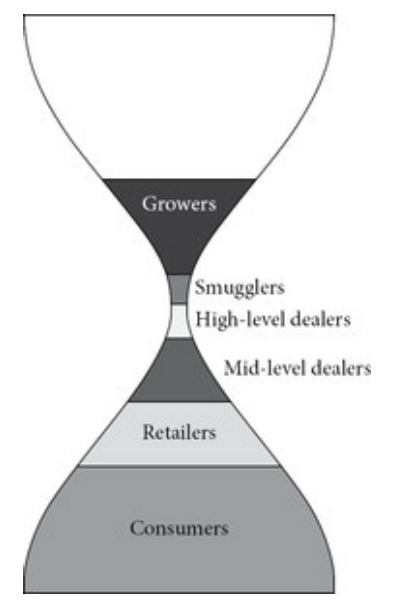
\includegraphics[width=0.3\textwidth,height=\textheight]{../chicago/figs/Reuter_hourglass.png}
\caption{Source: Reuter (2013)}
\end{figure}

\end{frame}

\begin{frame}{Cocaine}
\protect\hypertarget{cocaine}{}

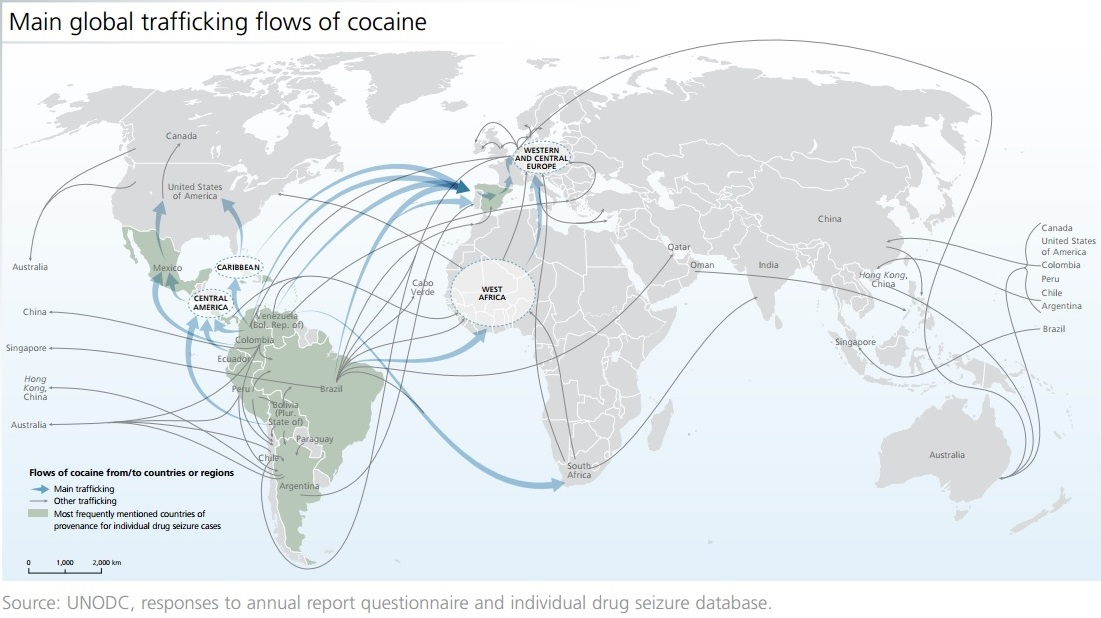
\includegraphics{../chicago/figs/cocaine_supply_map.jpg}

\end{frame}

\begin{frame}{Heroin}
\protect\hypertarget{heroin}{}

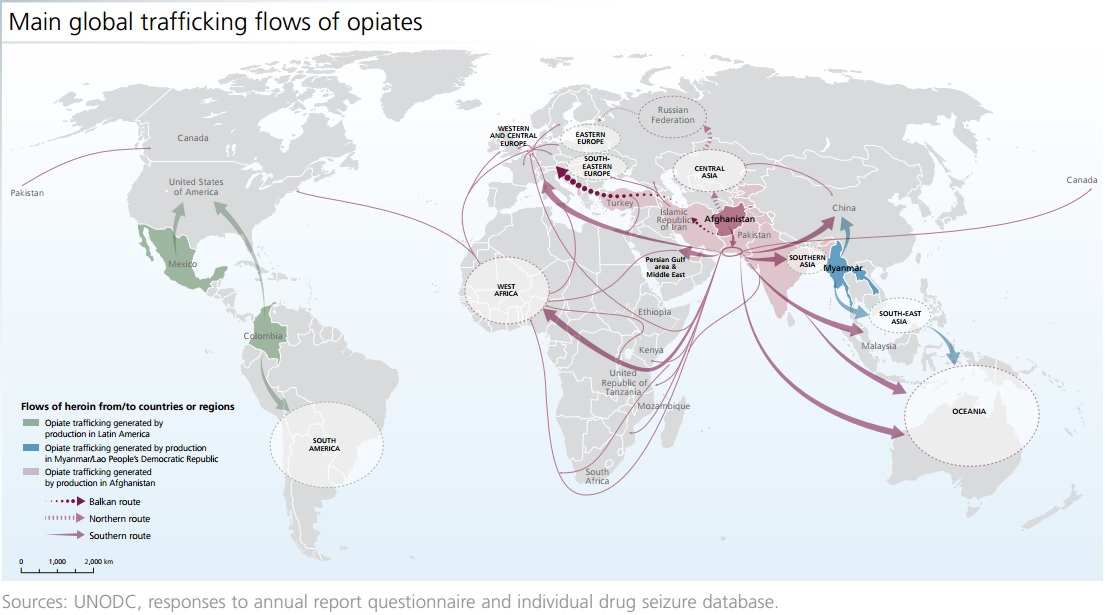
\includegraphics{../chicago/figs/opium_supply_map.jpg}

\end{frame}

\begin{frame}{Cost-Price Margins (Reuter 2013)}
\protect\hypertarget{cost-price-margins-reuter2010}{}

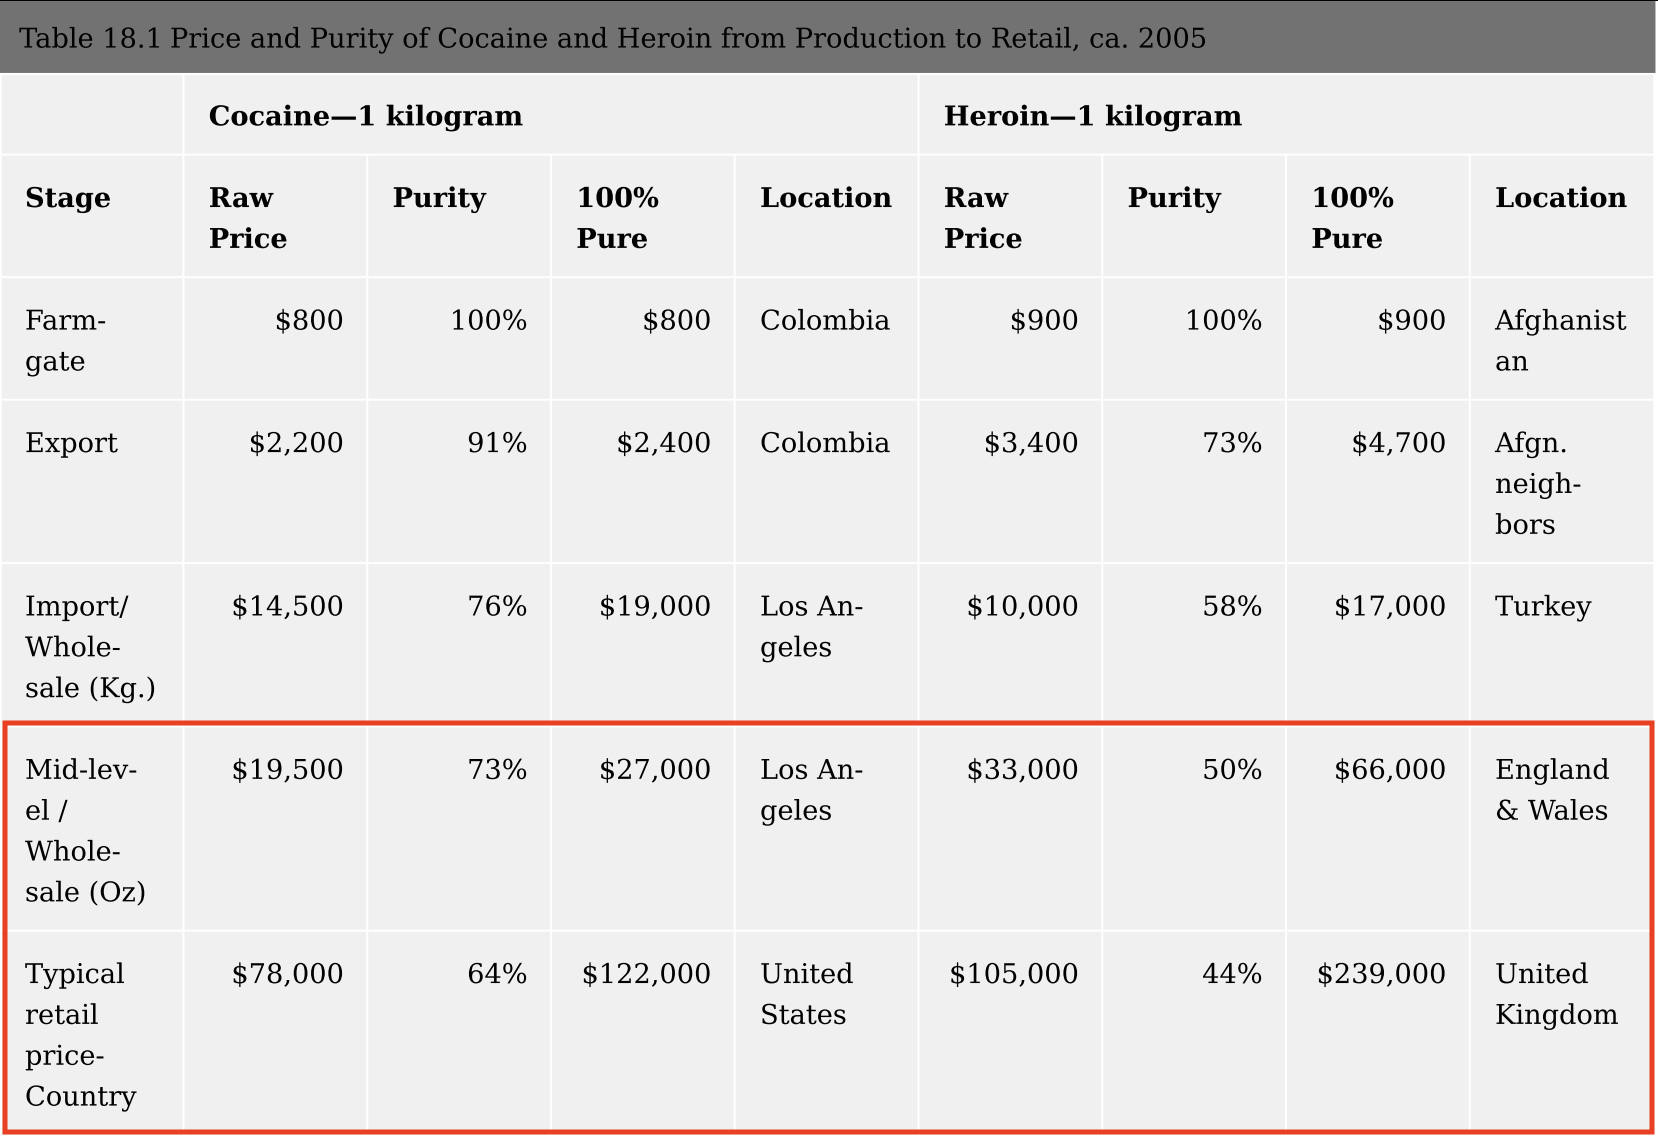
\includegraphics{../chicago/figs/Reuter_costprice.png}

\end{frame}

\begin{frame}{Retailers - Street Gangs}
\protect\hypertarget{retailers---street-gangs}{}

\begin{quote}
``Mexican DTOs and criminal groups are the principal transporters of
illicit drugs into and through the Chicago HIDTA region'' - DEA
\end{quote}

\begin{quote}
``Street gangs control most retail drug distribution in the
{[}Chicago{]} and are increasingly exploiting relationships with other
gangs or DTOs and use of technology to advance their criminal
activities'' - DEA
\end{quote}

\begin{itemize}
\tightlist
\item
  Some involvement in production (e.g.~converting powder to crack
  cocaine, repackaging)
\item
  Non-economic operating expenses dominate\ldots{}
\end{itemize}

\end{frame}

\begin{frame}{Operating Expenses}
\protect\hypertarget{operating-expenses}{}

\begin{figure}
\centering
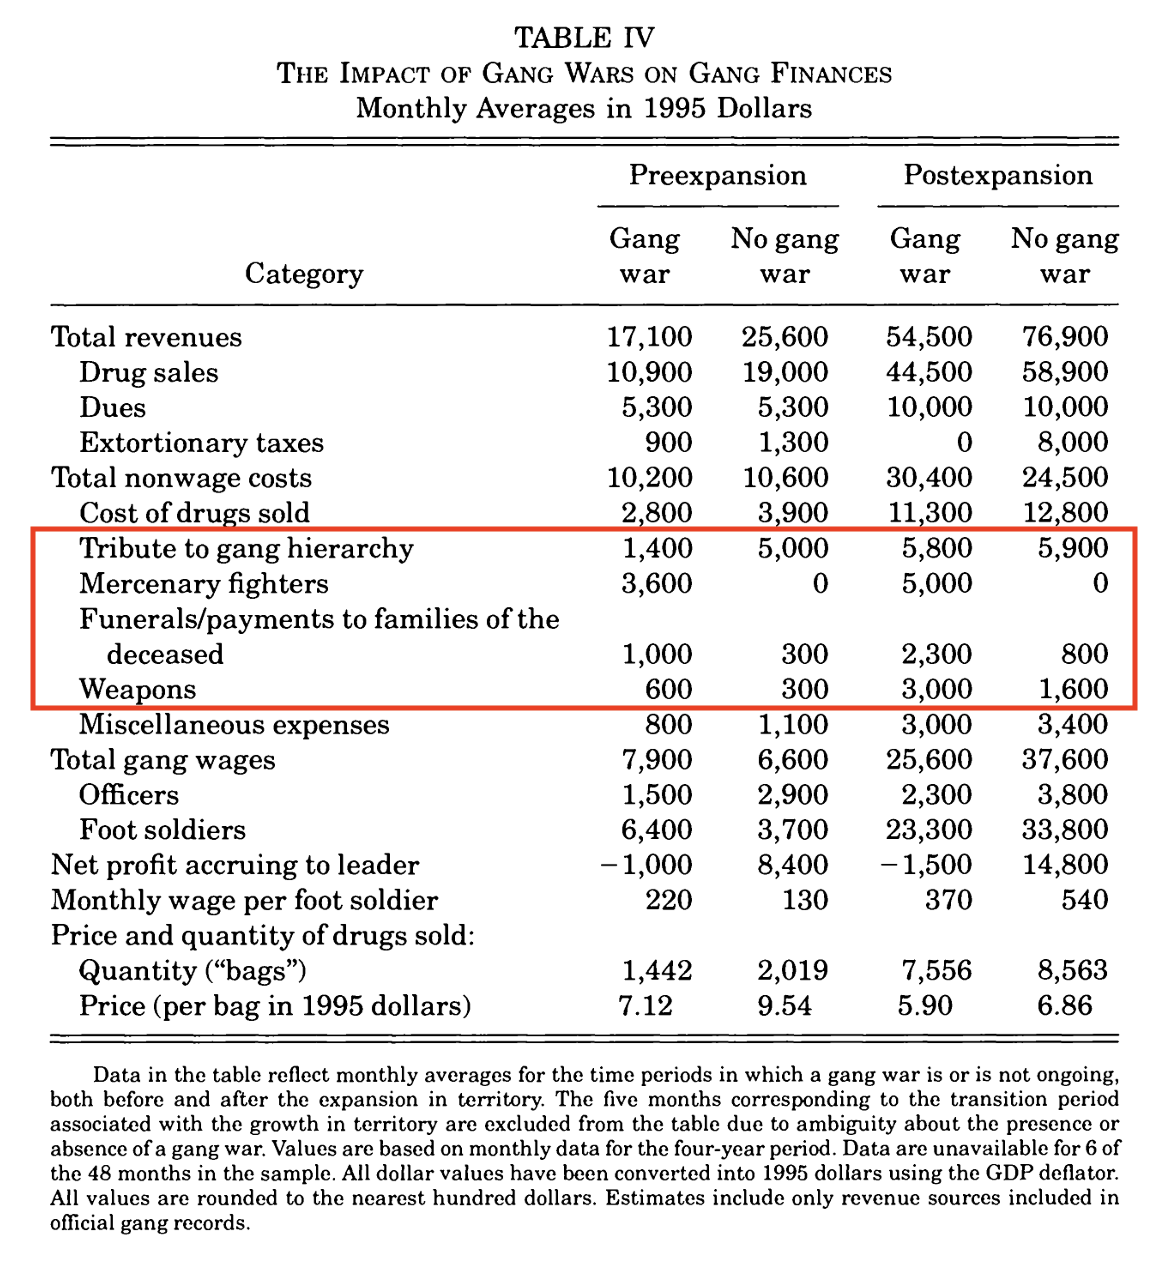
\includegraphics{../chicago/figs/lv_table4.png}
\caption{Source: Levitt and Venkatesh (2000), QJE}
\end{figure}

\end{frame}

\begin{frame}{Territoriality}
\protect\hypertarget{territoriality}{}

\begin{quote}
``If you want to expand your sales, you have to expand your street
corners. You know, you have to physically take street corners, which is
a violent act.'' - John Lippert, \emph{Bloomberg Markets}
\end{quote}

\begin{quote}
``Because crack distribution generates significant profits for street
gangs, low-level rival gang members routinely engage in violence to
acquire turf or steal drugs or drug proceeds'' - DEA
\end{quote}

\end{frame}

\begin{frame}{Territoriality}
\protect\hypertarget{territoriality-1}{}

\begin{figure}
\centering
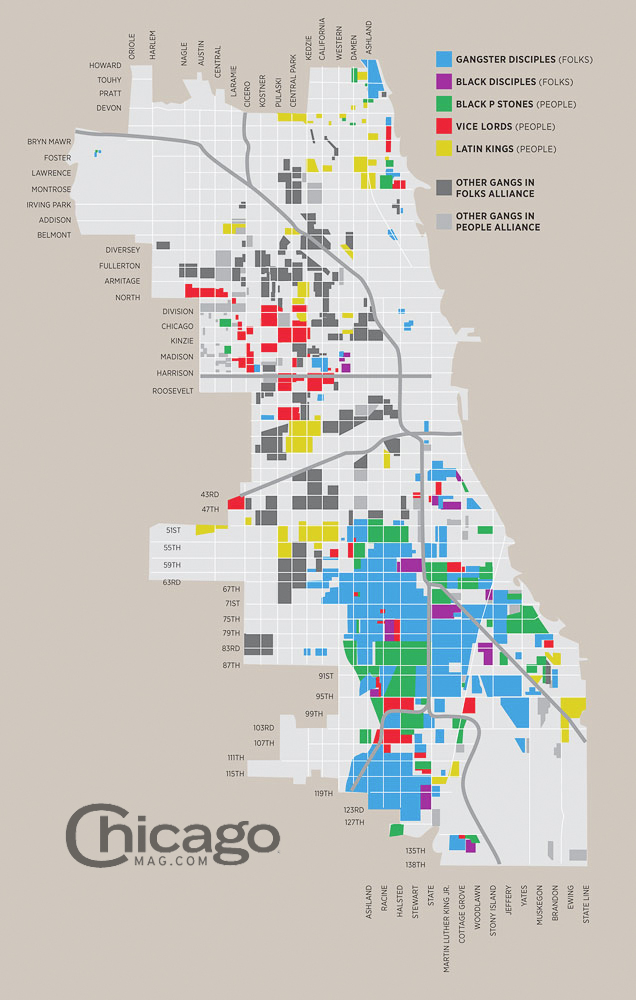
\includegraphics{../chicago/figs/gangmap2012cmag.jpg}
\caption{Sources: Chicago Crime Commission Gang Book 2012, \emph{Chicago
Magazine}}
\end{figure}

\end{frame}

\begin{frame}{Price and Violent Competition}
\protect\hypertarget{price-and-violent-competition}{}

\textbf{Gang Wars}

\begin{itemize}
\tightlist
\item
  Levitt and Venkatesh (2000)

  \begin{itemize}
  \tightlist
  \item
    Gang wars occur about 25 percent of the time
  \item
    Gang wars result in 20-30 percent drop in prices and quantities sold
  \item
    Death rate (annual) for members: 7 percent
  \end{itemize}
\item
  Papachristos (2009)

  \begin{itemize}
  \tightlist
  \item
    35 percent of homicides in 1994, 1998, 2002 documented as
    gang-related by homicide detectives
  \item
    88 percent inter-gang
  \end{itemize}
\end{itemize}

\begin{quote}
``In 2006 nearly 50 percent of the homicides and a large percentage of
other violent crimes and property crimes committed in Chicago were
attributed to street gangs that are involved in drug trafficking'' - DEA
\end{quote}

\textbf{Law Enforcement and Imprisonment}

\begin{quote}
``3,500 of the 13,000 inmates currently housed in the Cook County Jail
have some gang affiliation'' - DEA
\end{quote}

\begin{itemize}
\tightlist
\item
  At any given time, 1/3 of gang leadership is imprisoned (Levitt and
  Venkatesh 2000)
\end{itemize}

\end{frame}

\begin{frame}{Homicides and Non-Fatal Shootings}
\protect\hypertarget{homicides-and-non-fatal-shootings}{}

\begin{figure}
\centering
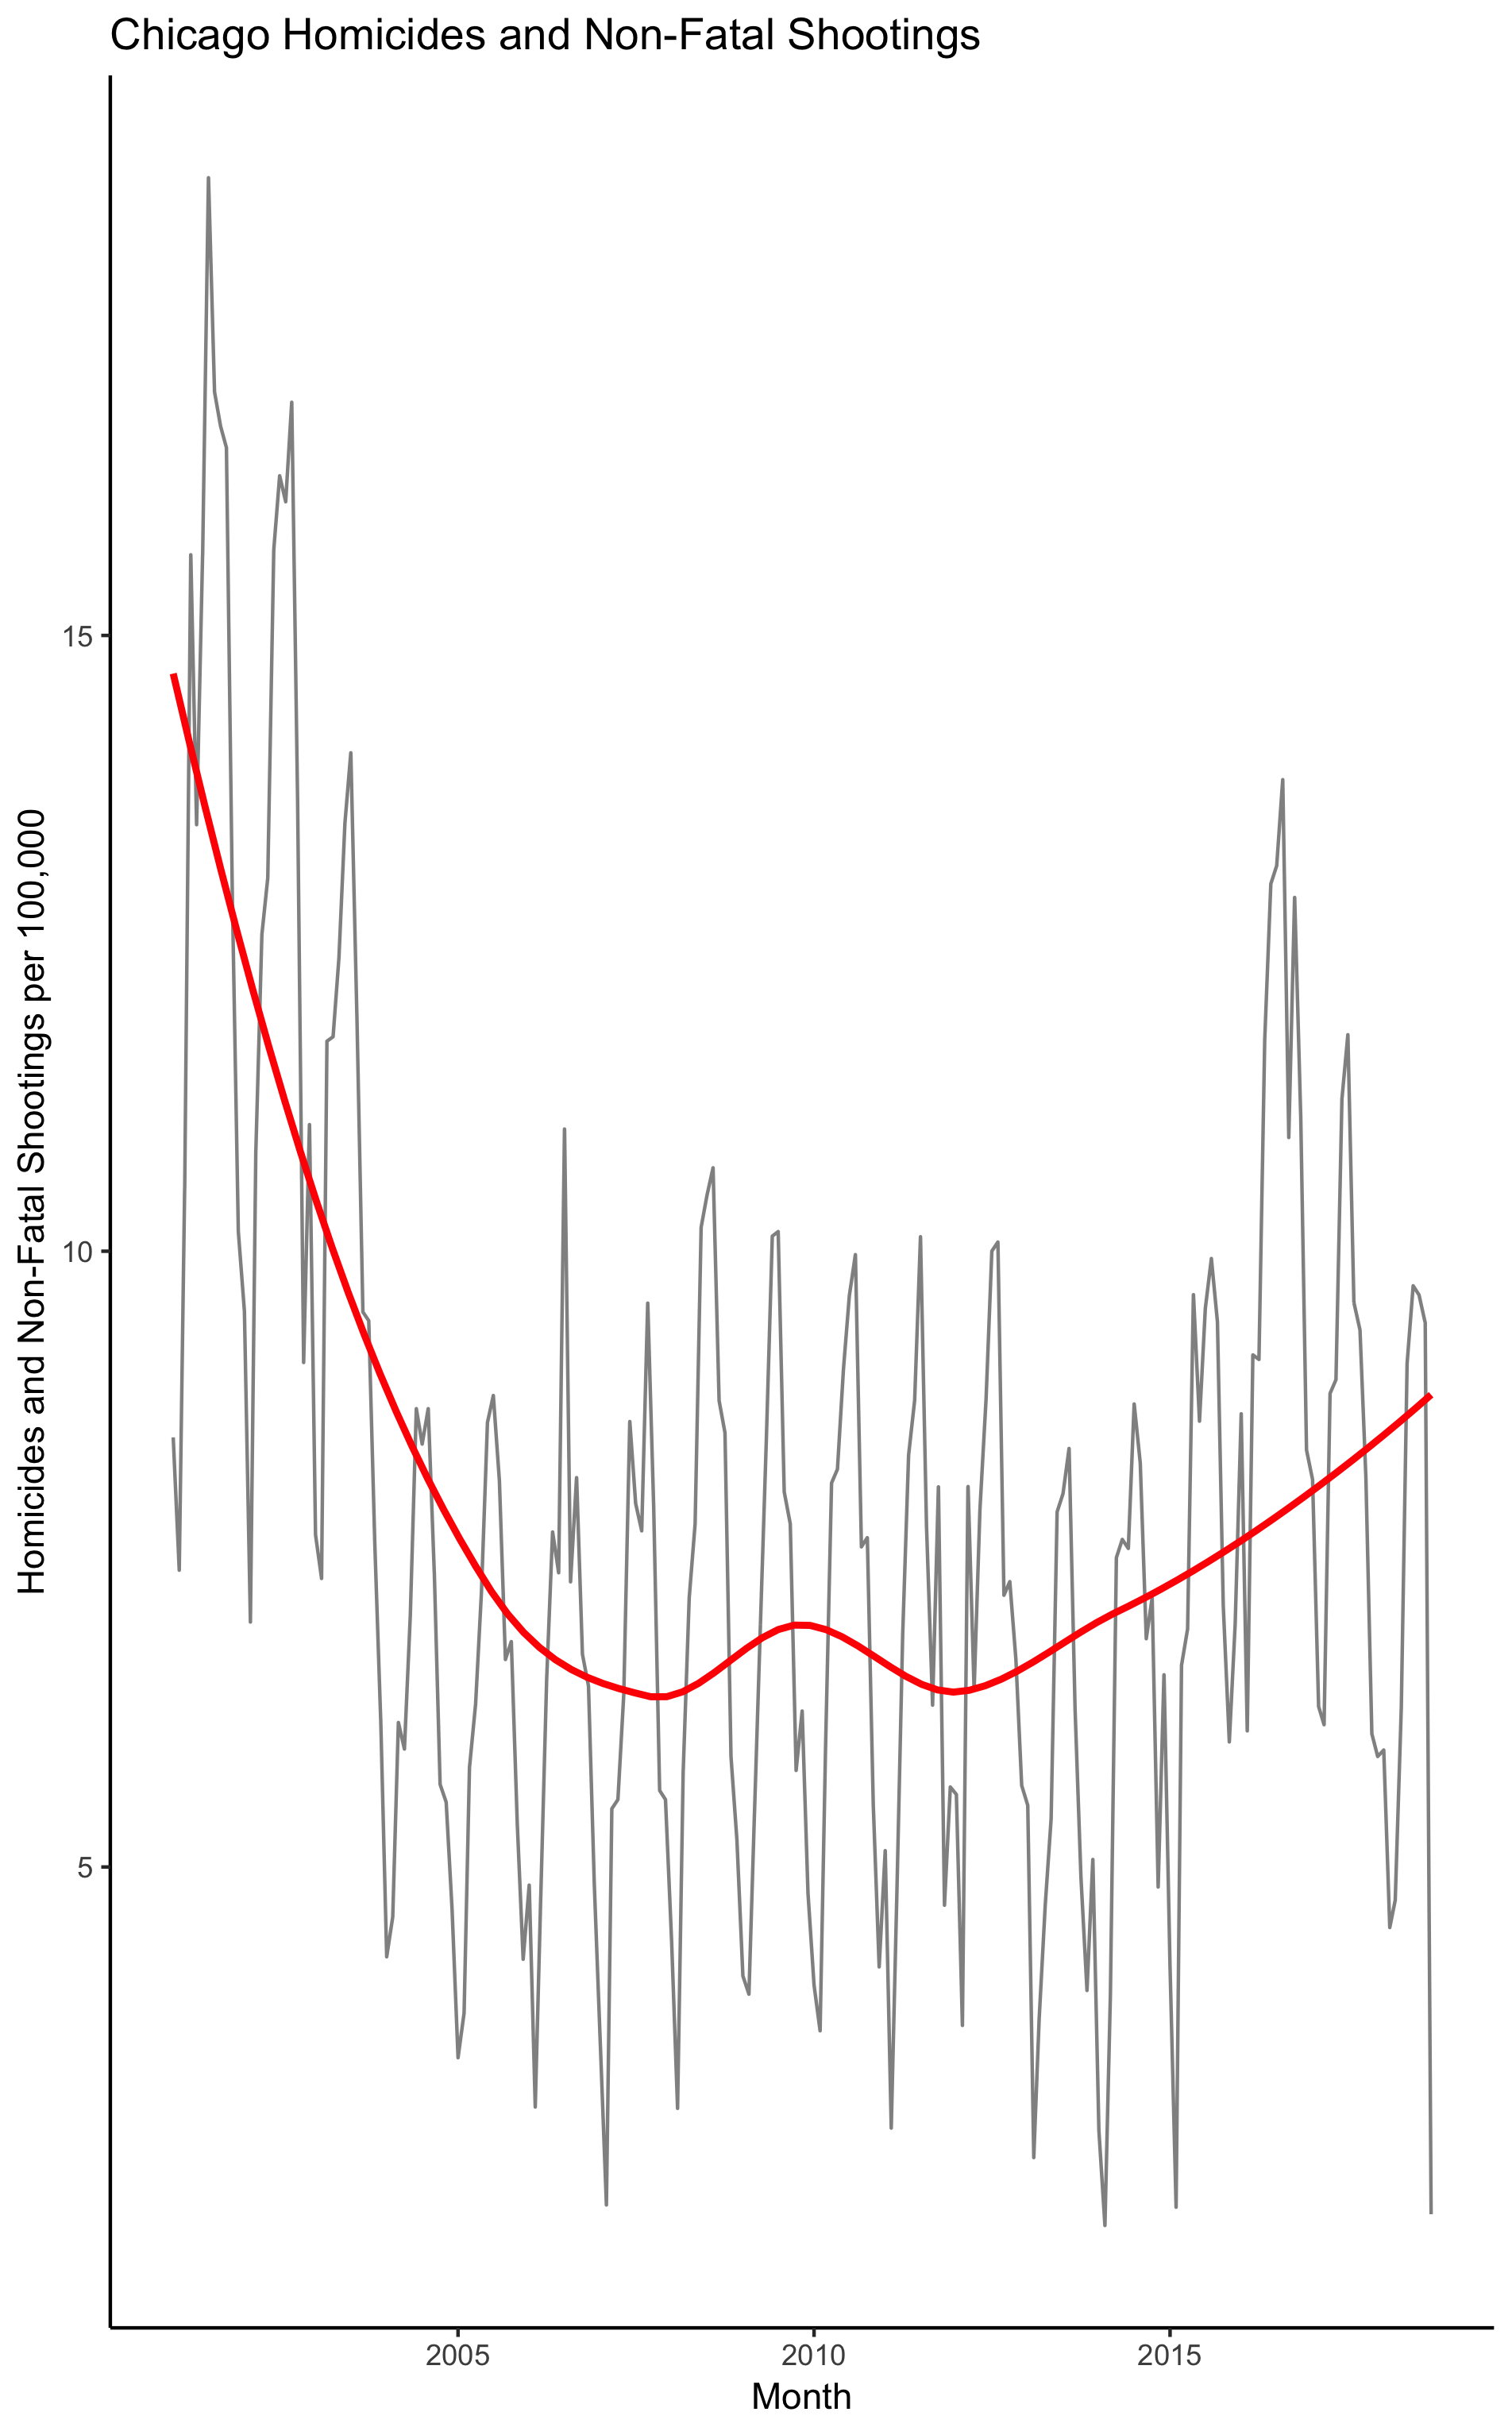
\includegraphics{../chicago/figs/hnfs_t_plot.png}
\caption{Source: Chicago PD}
\end{figure}

\end{frame}

\begin{frame}{Homicides and Non-Fatal Shootings}
\protect\hypertarget{homicides-and-non-fatal-shootings-1}{}

\begin{figure}
\centering
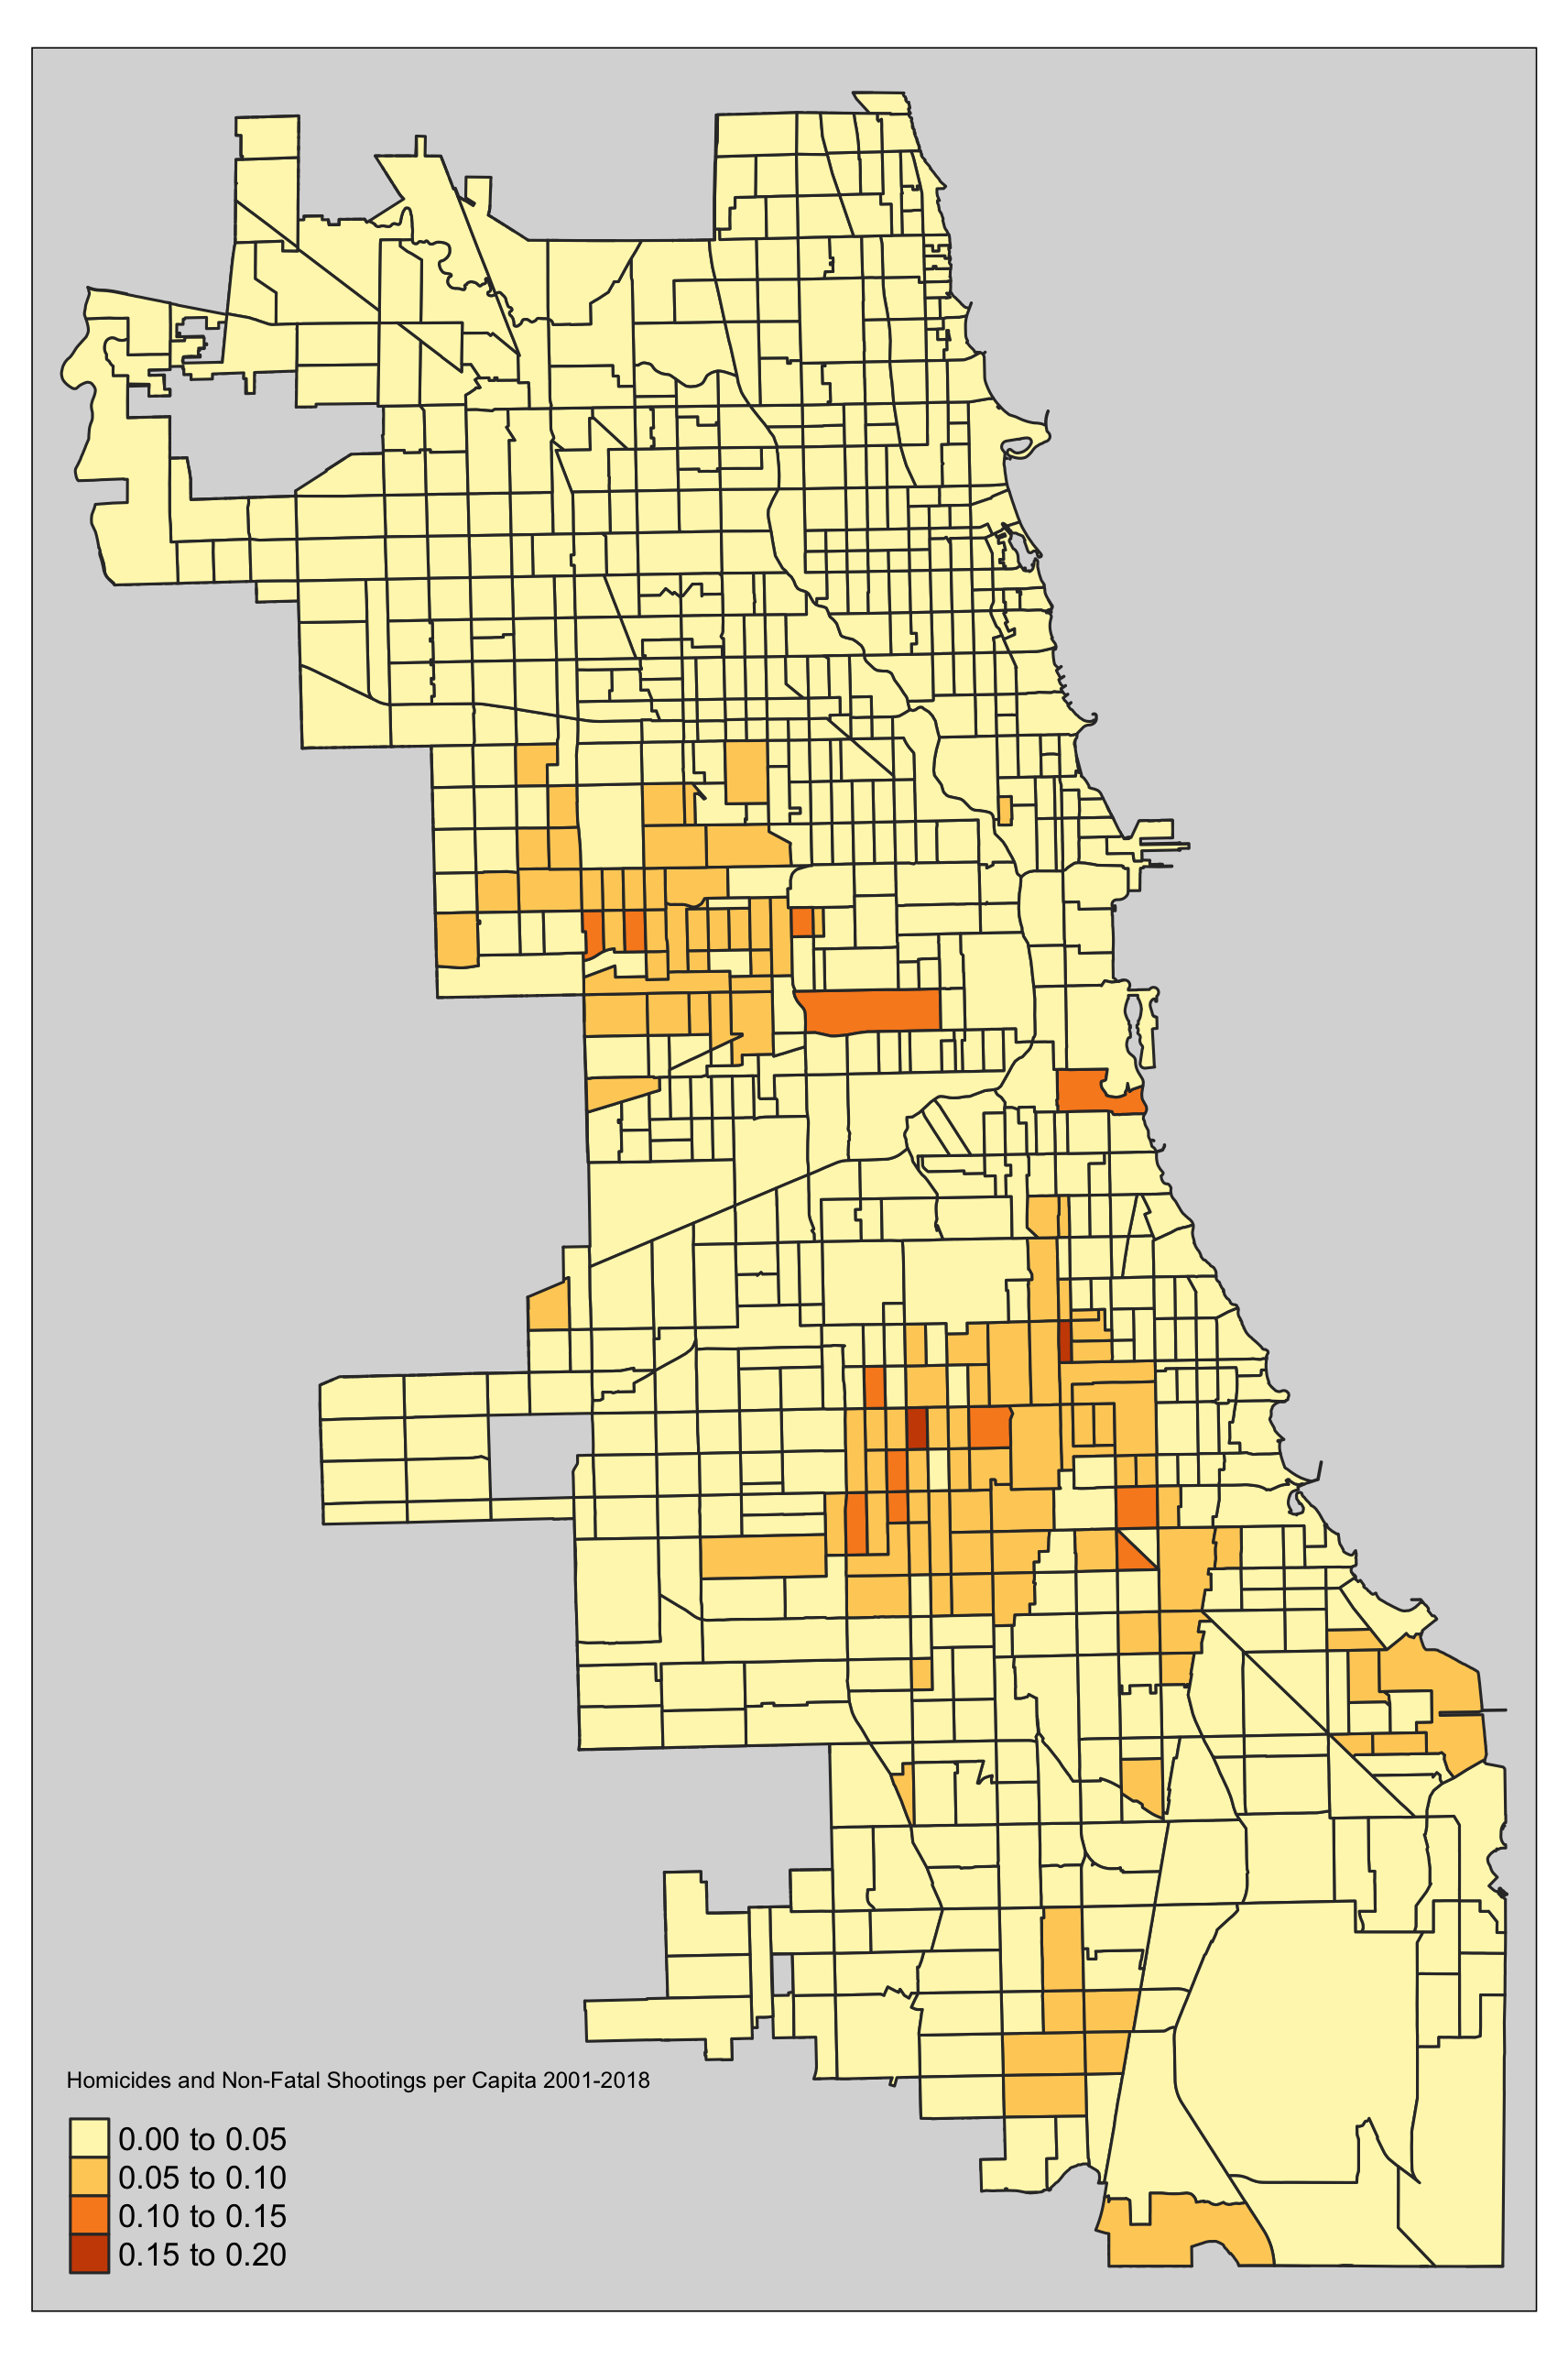
\includegraphics{../chicago/figs/chi_tsa_map.png}
\caption{Source: Chicago PD}
\end{figure}

\end{frame}

\begin{frame}{Narcotics Arrests}
\protect\hypertarget{narcotics-arrests}{}

\begin{figure}
\centering
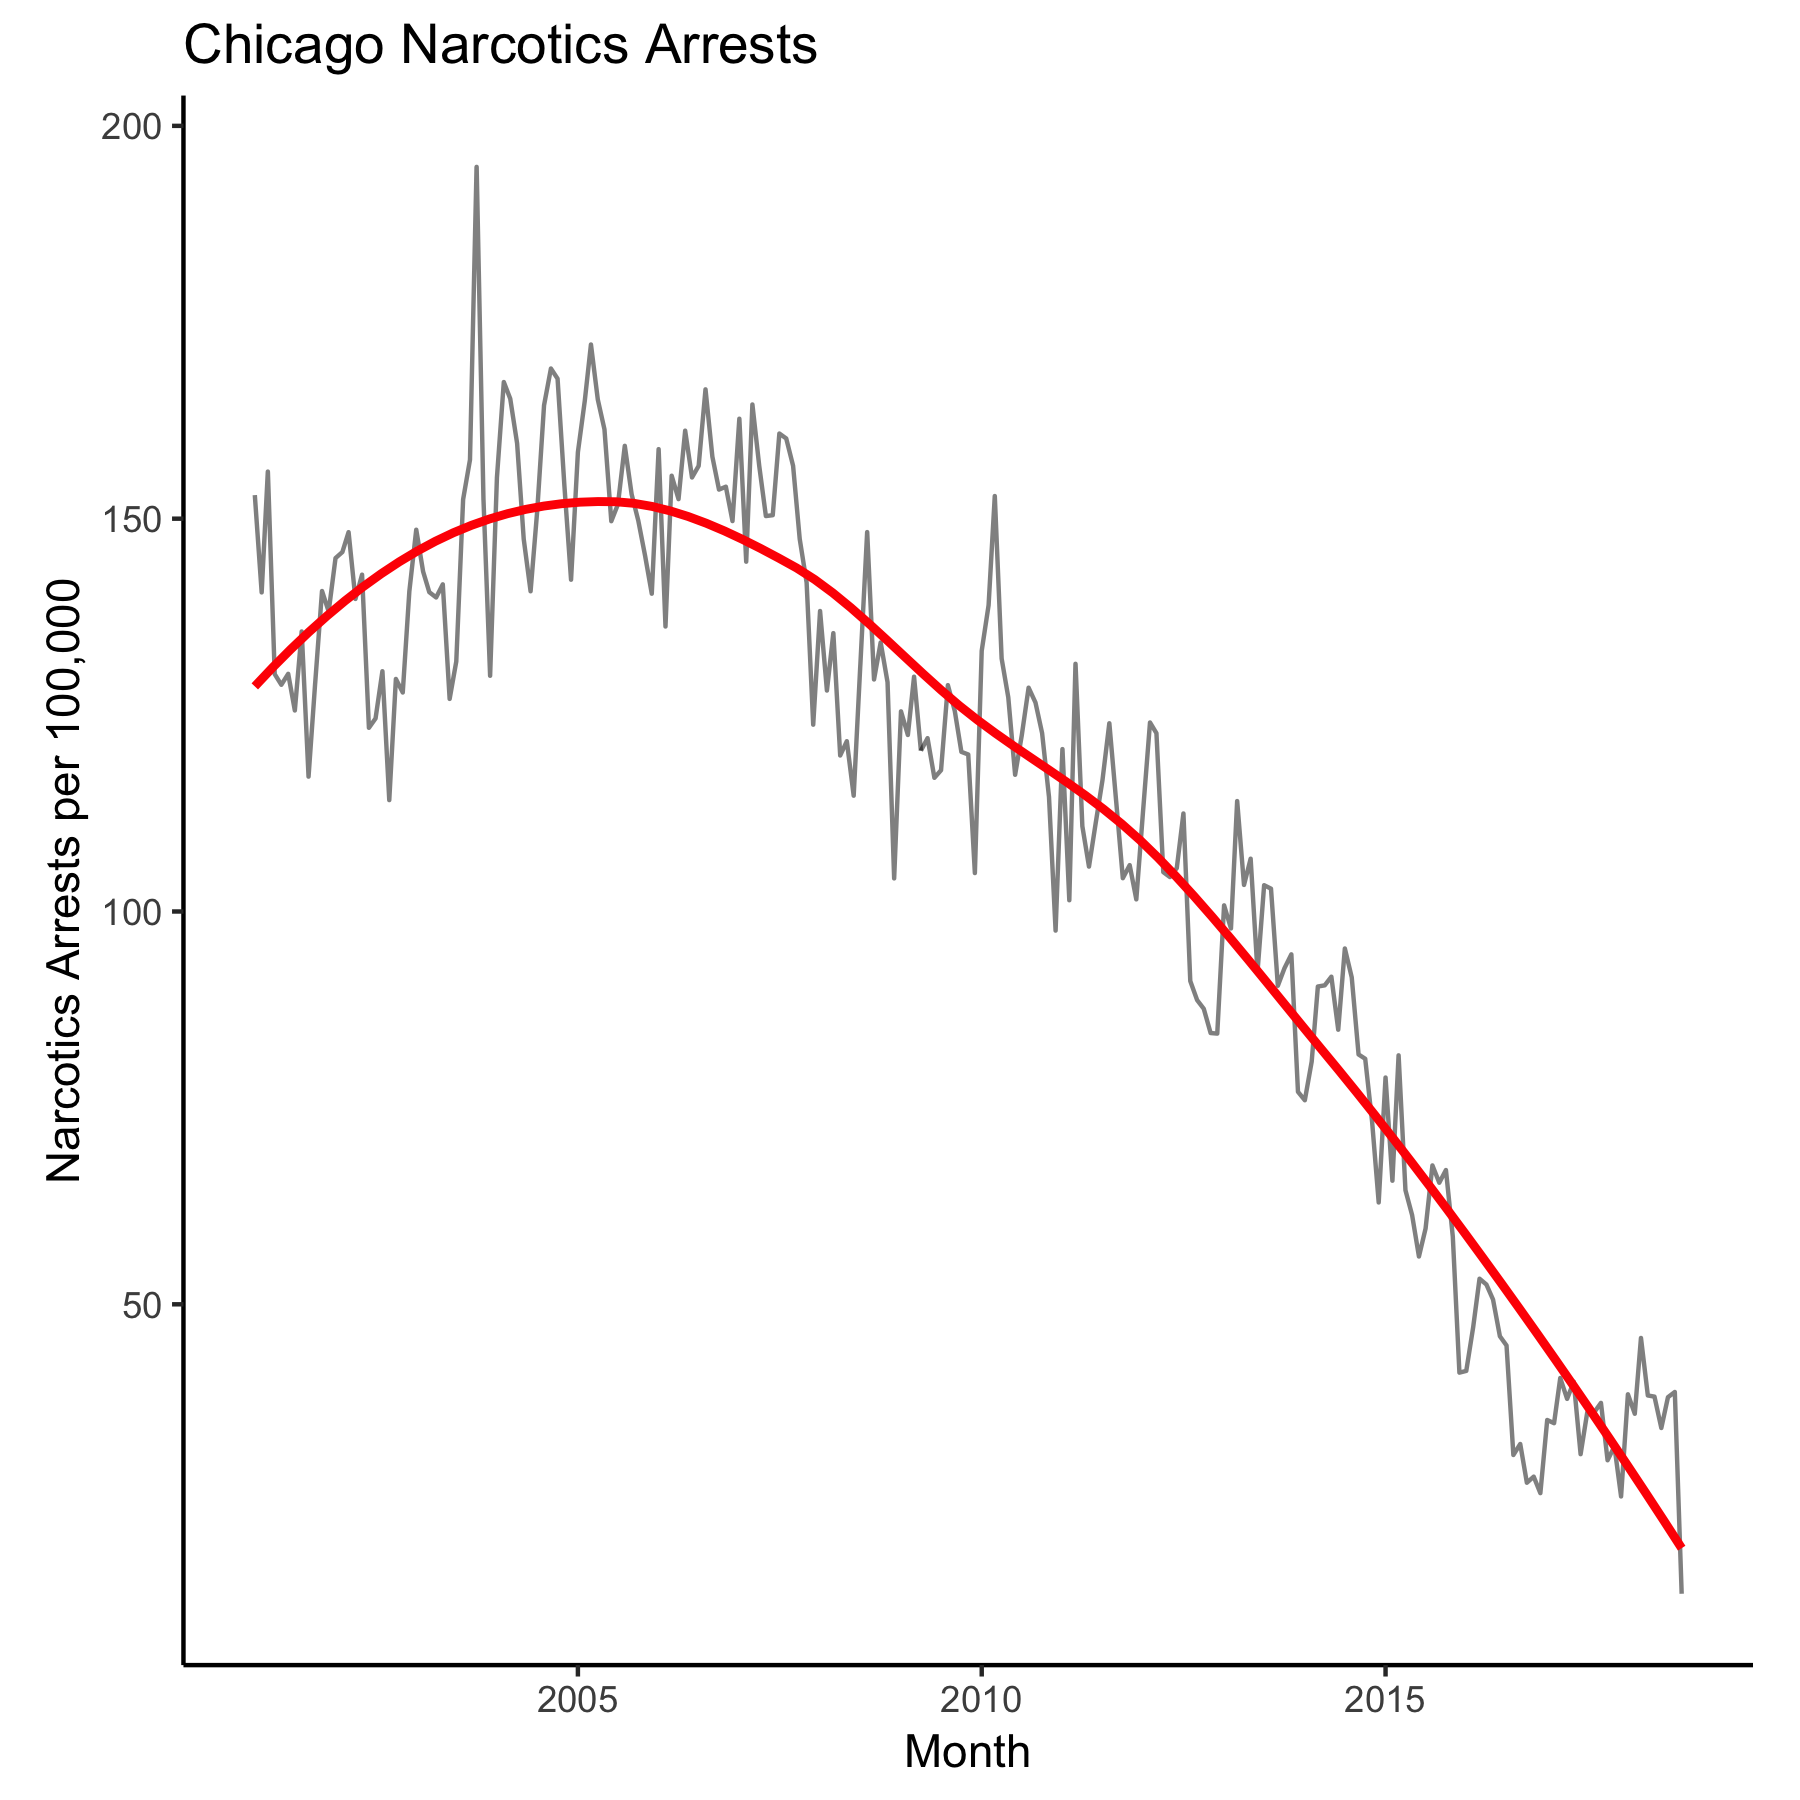
\includegraphics{../chicago/figs/narcotics_t_plot.png}
\caption{Source: Chicago PD}
\end{figure}

\end{frame}

\begin{frame}{Narcotics Arrests}
\protect\hypertarget{narcotics-arrests-1}{}

\begin{figure}
\centering
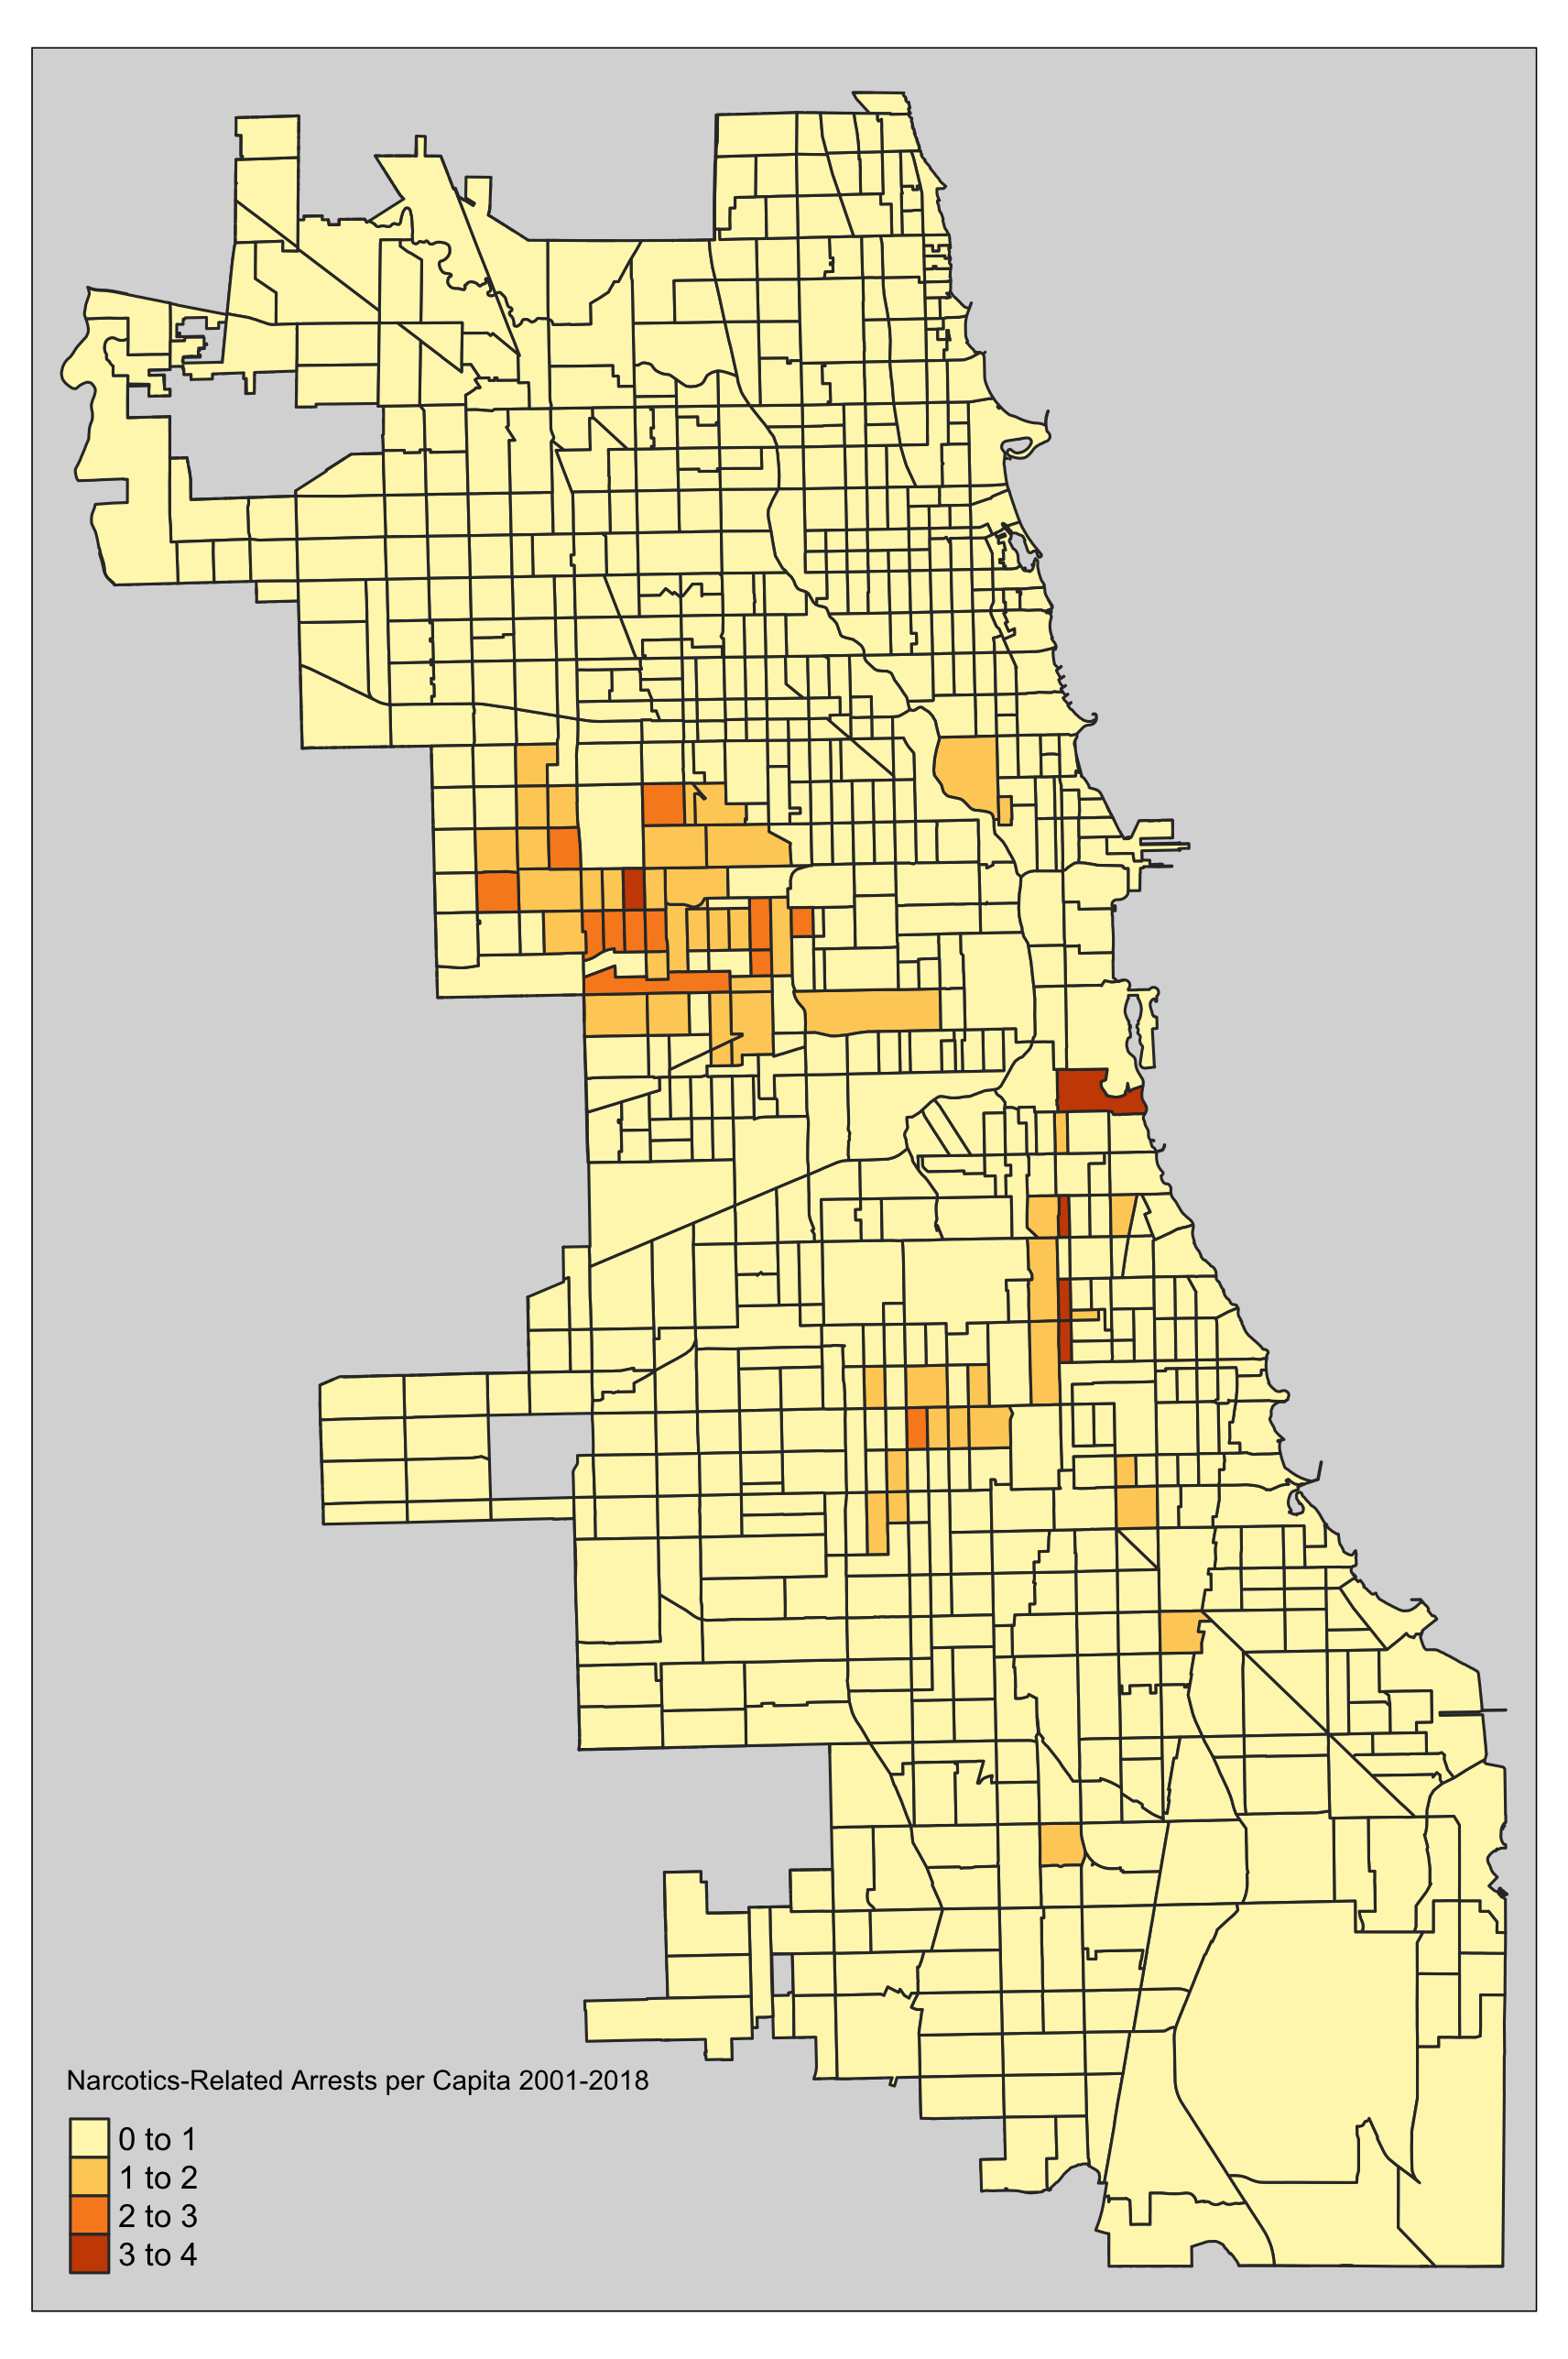
\includegraphics{../chicago/figs/chi_tna_map.png}
\caption{Source: Chicago PD}
\end{figure}

\end{frame}

\begin{frame}{Questions}
\protect\hypertarget{questions}{}

\textbf{Labor Market for Retailers}

\begin{itemize}
\tightlist
\item
  If retail prices are so high, why are earnings for dealers so low?
\item
  Why is compensation so low, given risk?
\end{itemize}

\textbf{Territoriality and Competition}

\begin{itemize}
\tightlist
\item
  Why is violence so uniquely associated with black markets?
\item
  Violence versus prices as competitive means\ldots complements or
  substitutes?
\item
  Consumers presumably can travel quickly to different
  territories\ldots what benefits does `turf' bring if not market power?
\end{itemize}

\textbf{Policy}

\begin{itemize}
\tightlist
\item
  How would increased police enforcement (seizures or arrests) affect
  competition (price and violent) between groups?
\item
  Radical counterfactual: drug legalization

  \begin{itemize}
  \tightlist
  \item
    Tradeoff(?): violence versus consumption
  \end{itemize}
\end{itemize}

\end{frame}

\begin{frame}{References}
\protect\hypertarget{references}{}

\hypertarget{refs}{}
\leavevmode\hypertarget{ref-Levitt2000}{}%
Levitt, Steven D, and Sudhir Alladi Venkatesh. 2000. ``An economic
analysis of a drug-selling gang's finances.'' \emph{Quarterly Journal of
Economics}, 755--89.

\leavevmode\hypertarget{ref-Papachristos2009}{}%
Papachristos, Andrew V. 2009. ``Murder by Structure: Dominance Relations
and the Social Structure of Gang Homicide.'' \emph{American Journal of
Sociology} 115 (1): 74--128.

\leavevmode\hypertarget{ref-Reuter2010}{}%
Reuter, Peter. 2013. ``Drug Markets and Organized Crime,'' no. August:
1--15.

\leavevmode\hypertarget{ref-UNODC2011}{}%
``World Drug Report.'' 2011. UNODC2011.

\end{frame}


%\section[]{}
%\frame{\small \frametitle{Table of Contents}
%\tableofcontents}
\end{document}
